\documentclass{article}

\usepackage{amsmath}
\usepackage{booktabs}
\usepackage{array}
\usepackage{longtable}
\usepackage{xcolor}
\usepackage{listings}
\usepackage{float}
\usepackage{tikz}
\usetikzlibrary{arrows.meta,positioning,fit,calc,backgrounds}
\usepackage{pgfplots}
\pgfplotsset{compat=1.16}
\usepackage[hidelinks]{hyperref}

\lstset{basicstyle=\ttfamily\footnotesize, frame=single, keepspaces=true,
        showstringspaces=false}

% ---------- TikZ styles used in all diagrams ----------
\tikzset{
  wbox/.style={draw, rounded corners=2pt, align=center, font=\footnotesize,
               inner sep=4pt, fill=blue!7},
  dbox/.style={draw, rounded corners=7pt, align=center, font=\footnotesize,
               inner sep=4pt, fill=green!10},
  ext/.style={draw, dashed, align=center, font=\footnotesize,
              inner sep=4pt, fill=gray!10},
  arr/.style={-{Stealth[length=2mm]}, thick},
  call/.style={circle, draw=red!70!black, fill=white, inner sep=1pt,
               font=\tiny\bfseries, text=red!70!black},
}

% ---------- Illustrative field used in the mock-up plots ----------
% Two smooth "hills" (synthetic data, NOT real measurements).
% Isoline radii were computed for levels 0.5, 1.0, 1.5, 2.0, 2.5.
\newcommand{\isoTwoD}[3]{%
  \addplot[domain=0:360, samples=61, thick, black]
    ({#1+#3*cos(x)},{#2+#3*sin(x)});}
\newcommand{\isoThreeD}[4]{%
  \addplot3[domain=0:360, samples=61, samples y=0, thick, black]
    ({#1+#3*cos(x)},{#2+#3*sin(x)},{#4+0.04});}

\newcommand{\hillThreeD}[2]{%
\begin{tikzpicture}
\begin{axis}[width=#1, height=#2, view={-40}{28},
  xlabel={$x$ [m]}, ylabel={$y$ [m]}, zlabel={value},
  xmin=0, xmax=100, ymin=0, ymax=100, zmin=0, zmax=3.5,
  tick label style={font=\tiny}, label style={font=\scriptsize},
  xtick={0,50,100}, ytick={0,50,100}, ztick={0,1,2,3}]
\addplot3[surf, shader=interp, opacity=0.8, samples=26,
          domain=0:100, y domain=0:100]
  {3*exp(-((x-25)^2+(y-70)^2)/200) + 2*exp(-((x-72)^2+(y-30)^2)/338)};
\isoThreeD{25}{70}{18.93}{0.5}
\isoThreeD{25}{70}{14.82}{1.0}
\isoThreeD{25}{70}{11.77}{1.5}
\isoThreeD{25}{70}{9.00}{2.0}
\isoThreeD{25}{70}{6.04}{2.5}
\isoThreeD{72}{30}{21.65}{0.5}
\isoThreeD{72}{30}{15.31}{1.0}
\isoThreeD{72}{30}{9.86}{1.5}
\addplot3[only marks, mark=star, mark size=3pt, thick, red]
  coordinates {(25,70,3.1) (72,30,2.1)};
\end{axis}
\end{tikzpicture}}

\newcommand{\hillTwoD}[1]{%
\begin{tikzpicture}
\begin{axis}[width=#1, height=#1, xmin=0, xmax=100, ymin=0, ymax=100,
  xlabel={$x$ [m]}, ylabel={$y$ [m]},
  tick label style={font=\tiny}, label style={font=\scriptsize},
  xtick={0,50,100}, ytick={0,50,100}]
\addplot[gray!70, thin] coordinates {(5,10) (95,10) (95,20) (5,20) (5,30)
  (95,30) (95,40) (5,40) (5,50) (95,50) (95,60) (5,60) (5,70) (95,70)
  (95,80) (5,80) (5,90) (95,90)};
\isoTwoD{25}{70}{18.93}
\isoTwoD{25}{70}{14.82}
\isoTwoD{25}{70}{11.77}
\isoTwoD{25}{70}{9.00}
\isoTwoD{25}{70}{6.04}
\isoTwoD{72}{30}{21.65}
\isoTwoD{72}{30}{15.31}
\isoTwoD{72}{30}{9.86}
\addplot[only marks, mark=star, mark size=3pt, thick, red]
  coordinates {(25,70) (72,30)};
\end{axis}
\end{tikzpicture}}

\title{UKRAINIX WATERDRONE\\[2mm]
       Software Repository and Data Analysis App\\[2mm]
       \large Onboarding Guide for New Team Members}
\author{UKRAINIX WATERDRONE project}
\date{2 November 2026}

\begin{document}

\maketitle
\tableofcontents

% =====================================================================
\section{Introduction}
\label{sec:intro}

This guide is written for new members of the UKRAINIX WATERDRONE team.
It explains

\begin{itemize}
\item how the \path{waterdrone-software} repository is organised
      (Section~\ref{sec:repo});
\item what the data analysis app is for, which features it will have and how
      data flows through it (Section~\ref{sec:app});
\item how the finished app is expected to look on screen
      (Section~\ref{sec:screens});
\item how the app is tested in three phases (Section~\ref{sec:tests});
\item what is still undecided and where a newcomer can start
      (Section~\ref{sec:status}).
\end{itemize}

\subsection{Project status}

\textbf{The app does not exist yet.} At the time of writing
(2 November 2026) the folders of \path{analysis-app} have been created, each
leaf folder holds only a \path{.gitkeep} placeholder, and no Python script,
\path{__init__.py} or \path{pyproject.toml} has been written. Everything in
this guide therefore describes the agreed \emph{design}. File names, function
groups and screens are plans, and every picture that looks like a screenshot
is a mock-up drawn with invented data.

An earlier draft of the layout used more folders than the current one. If you
see any of the folders \path{tests}, \path{config/defaults},
\path{config/physics_models}, \path{geo}, \path{mesh}, \path{utils},
\path{state}, \path{physics/models} or \path{gui/widgets} inside
\path{analysis-app}, they are leftovers of that draft and are to be deleted
(the files with the same names, such as \path{physics/models.py}, are part of
the current plan).

\subsection{Glossary}

{\small
\begin{longtable}{@{}p{0.27\textwidth}p{0.68\textwidth}@{}}
\toprule
\textbf{Term} & \textbf{Meaning}\\
\midrule
\endhead
Waterdrone & The drone platform that logs its GPS position and
  concentration-related sensor readings into a CSV file.\\
Parameter & Any measured quantity, i.e.\ every CSV column whose name is in
  capital letters and that is not one of the fixed columns
  (Section~\ref{sec:csv}).\\
Sample & One parsed CSV file: a list of points with time, local position
  and one value per parameter.\\
Local Cartesian coordinates & Position in metres $(x,y)$ relative to a shared
  reference origin, computed from latitude and longitude.\\
Control points & A small set of locations that the drone visits quickly, so
  that the readings there are effectively a snapshot in time.\\
Normalization sample & The sample made of control points; it serves as the
  first reference for normalization.\\
Normalization chain & Ordered list of samples in which each sample is
  normalized against the previous normalized one.\\
Triangulation (mesh) & Triangles connecting the sample points; the basis for
  interpolation and isolines.\\
Isoline & A line connecting positions of equal parameter value.\\
Origin & A point from which the measured field spreads, found by fitting a
  physics model to the data.\\
Physics model & A forward model that computes the field produced by a given
  set of origins; chosen per parameter in a dictionary text file.\\
\bottomrule
\end{longtable}
}

% =====================================================================
\section{Repository structure}
\label{sec:repo}

The repository \path{waterdrone-software} is to be published on GitHub. It
holds a data analysis app, the test data for that app, and (later) a second
app. The layout is:

\noindent\begin{minipage}{\textwidth}
\begin{lstlisting}
waterdrone-software/
|-- analysis-app/          data analysis app (Python)
|   |-- README.md
|   |-- config/            physics_models.txt, defaults.txt
|   |-- docs/
|   `-- src/analysis_app/  the Python package
|-- samples/               all test data and scripts
|   |-- phase1_synthetic/  from the app's physics model
|   |   `-- scripts/
|   |-- phase2_real/       real-world data
|   |   |-- raw/           open-source data as downloaded
|   |   |-- reduced/       converted to waterdrone CSV
|   |   `-- scripts/
|   `-- phase3_normalization/  (not created yet)
`-- (configurator app)     planned, not created yet
\end{lstlisting}
\end{minipage}

\begin{center}
\begin{tabular}{@{}p{0.25\textwidth}p{0.70\textwidth}@{}}
\toprule
\textbf{Part} & \textbf{Purpose}\\
\midrule
\path{analysis-app/} & Reads waterdrone CSV files and turns them into
  normalized samples, isolines, field origins and an interactive 3D plot.
  Written as functional Python (no classes). Described in detail in
  Section~\ref{sec:app}.\\
\path{samples/} & The only place for test data. The analysis app has no
  \path{tests/} folder of its own: all testing uses the three sample folders
  (Section~\ref{sec:tests}).\\
Configurator app & A second app for configuring the waterdrone itself. It is
  planned for later; nothing exists yet.\\
\bottomrule
\end{tabular}
\end{center}

\subsection{The waterdrone CSV format}
\label{sec:csv}

Every sample, synthetic or real, uses the same CSV format.

\begin{itemize}
\item \texttt{TIMESTAMP} -- integer, the computer time at which the row was
      logged.
\item \texttt{LATITUDE}, \texttt{LONGITUDE} -- position in degrees.
\item \texttt{Z} -- measurement depth, when present. It is \emph{not} the
      vertical axis of the plot (Section~\ref{sec:viz}).
\item All other columns are parameters. Their names are written in capital
      letters. Only concentration-related quantities are kept; absolute-value
      quantities are not part of the format.
\end{itemize}

The app detects the fixed columns and treats every remaining capitalised
column as a parameter, so the number of parameters is not fixed in advance.
A made-up example:

\begin{lstlisting}
TIMESTAMP,LATITUDE,LONGITUDE,Z,PARAM_A,PARAM_B
1730500000,50.00010,30.00020,0.5,12.4,0.83
1730500001,50.00011,30.00022,0.5,12.6,0.80
1730500002,50.00013,30.00025,0.5,13.1,0.79
\end{lstlisting}

% =====================================================================
\section{The data analysis app}
\label{sec:app}

\subsection{General task}

The waterdrone drives over a body of water and logs its position together
with concentration-related readings. The analysis app turns such a file into
a picture of how each measured quantity is distributed over the water. For
every parameter it

\begin{enumerate}
\item converts the GPS track into local Cartesian coordinates in metres;
\item optionally \emph{normalizes} the readings against a quick reference
      survey, so that long surveys or several surveys become comparable;
\item builds a triangulated map of the normalized readings and extracts
      \emph{isolines} from it;
\item finds the \emph{origins} of the field by least-squares fitting of a
      physics model;
\item shows readings, isolines and origins in an interactive 3D plot.
\end{enumerate}

\subsection{Planned features}

\begin{itemize}
\item \textbf{CSV import with validation.} Fixed columns and capitalised
      parameter columns are detected automatically. Rows with missing values
      (NaN), GPS glitches and duplicate timestamps are caught.
\item \textbf{Coordinate conversion.} Latitude and longitude become local
      $x,y$ in metres around a shared reference origin, together with an
      estimate of the projection error.
\item \textbf{Per-parameter computation.} Everything is computed for every
      parameter column, including each parameter's own normalization
      correction. The dropdown in the GUI only selects which result is shown.
\item \textbf{Chained normalization (optional).} A fast sample of several
      control points normalizes a big CSV; a still bigger sample can then be
      normalized against that result, and so on. The first step may be
      skipped.
\item \textbf{Triangulation and isolines.} Triangles that bridge gaps or land
      are dropped; isoline crossings are found on triangle edges and joined
      by a smoothing spline.
\item \textbf{Origin finding.} Multi-origin least-squares fit of a physics
      model, with bounds and diagnostics (RMS error, residual map, a sanity
      check of the number of origins, comparison with known origins on
      synthetic data).
\item \textbf{Pluggable physics models.} The model used for each parameter is
      named in a dictionary text file. Adding a model means adding one
      function and one dictionary entry; the solver is not touched.
\item \textbf{Configurable defaults.} Spline smoothing, isoline levels and
      similar settings live in a text file, not in the code.
\item \textbf{Interactive 3D visualization} in matplotlib, with a parameter
      dropdown and switches for the overlays.
\end{itemize}

\subsection{Design principles}
\label{sec:principles}

\begin{itemize}
\item \textbf{Functional Python, no OOP.} Pure functions with data passed
      explicitly. Data containers are plain \texttt{NamedTuple},
      \texttt{TypedDict} or numpy arrays without behaviour.
\item \textbf{One folder per concern, one file per group of related
      functions.} A file is roughly 150--400 lines. A file is split only when
      it stops being one coherent group; an outgrown file becomes a
      sub-package behind the same public names.
\item \textbf{Packages expose a public interface.} Each package's
      \path{__init__.py} re-exports its public functions, and other packages
      import from the package, never from its files. Files can then be
      reorganised without touching callers.
\item \textbf{Side effects at the edges.} File reading, GUI and plotting sit
      at the edges; \path{pipeline/} composes pure functions.
\item \textbf{Normalization before triangulation.} Isolines and origin fitting
      are always built on the \emph{normalized} sample, never on raw data.
\end{itemize}

\subsection{Package layout}
\label{sec:layout}

The Python package lives in \path{analysis-app/src/analysis_app/}:

\begin{lstlisting}
src/analysis_app/
|-- main.py              entry point: starts the GUI
|-- core/                types, config reader, functional helpers
|-- parsing/             CSV reading and validation, coordinates
|-- normalization/       matching, correction, chain
|-- isolines/            triangulation, contours
|-- physics/             model dictionary and forward models
|-- inversion/           least-squares origin fitting, diagnostics
|-- pipeline/            stages, run, state
|-- viz/                 3D plot and overlays
`-- gui/                 window, widgets, callbacks
\end{lstlisting}

The planned files (23 in total) and what each one groups together:

{\small
\begin{longtable}{@{}p{0.27\textwidth}p{0.69\textwidth}@{}}
\toprule
\textbf{File} & \textbf{Responsibility}\\
\midrule
\endhead
\path{main.py} & Entry point; starts the GUI.\\
\midrule
\multicolumn{2}{@{}l}{\textbf{\texttt{core/} -- shared foundations}}\\
\path{types.py} & Data containers (sample, mesh, isoline, origin, model spec,
  normalization result), CSV column-name constants, project exceptions.\\
\path{config.py} & Reader for the text/dictionary files, access to defaults,
  resolution of the config and samples paths.\\
\path{functional.py} & Compose/pipe helpers, per-parameter mapping, array
  helpers.\\
\midrule
\multicolumn{2}{@{}l}{\textbf{\texttt{parsing/} -- from CSV to a sample}}\\
\path{csv_parser.py} & Read the CSV, detect fixed columns and capitalised
  parameters, validate rows (NaN, GPS glitches, duplicate timestamps), build
  the sample.\\
\path{coordinates.py} & Choose the shared reference origin, convert
  latitude/longitude to local $x,y$ and back, estimate the projection
  error.\\
\midrule
\multicolumn{2}{@{}l}{\textbf{\texttt{normalization/} -- runs before isolines}}\\
\path{matching.py} & Extract control points, pair points of the big sample
  with them by distance and time, look up reference values at arbitrary
  points (spatial index).\\
\path{correction.py} & Fit and apply the time-dependence correction; residual
  check.\\
\path{chain.py} & Ordered, skippable chain; promote a normalized sample to
  be the reference grid of the next one.\\
\midrule
\multicolumn{2}{@{}l}{\textbf{\texttt{isolines/} -- works on normalized samples}}\\
\path{triangulation.py} & Triangulate; drop triangles bridging gaps or land;
  locate the triangle of a point; interpolate a value at a point.\\
\path{contours.py} & Choose levels, find edge crossings, link them into
  polylines, spline smoothing; isolines for one parameter.\\
\midrule
\multicolumn{2}{@{}l}{\textbf{\texttt{physics/} -- field models}}\\
\path{spec.py} & Load the model dictionary, map a CSV parameter to a model,
  bounds, validation.\\
\path{models.py} & Forward models: the field produced by given origins.
  May become a sub-package later.\\
\midrule
\multicolumn{2}{@{}l}{\textbf{\texttt{inversion/} -- finding the origins}}\\
\path{fit.py} & Initial guess, residuals, least-squares solve for several
  origins, parameter packing, bounds.\\
\path{diagnostics.py} & RMS, residual map, sanity check of the origin count,
  comparison with known origins (phase~1).\\
\midrule
\multicolumn{2}{@{}l}{\textbf{\texttt{pipeline/} -- composition}}\\
\path{stages.py} & Load, normalize, isoline and origin stages (inputs to
  result).\\
\path{run.py} & Run one or all parameters, result cache, optional
  parallelism.\\
\path{state.py} & Immutable app state plus pure update functions (add a
  sample, set the chain, select a parameter, store results).\\
\midrule
\multicolumn{2}{@{}l}{\textbf{\texttt{viz/} -- drawing}}\\
\path{plot3d.py} & 3D axes, surface/points, labels and style.\\
\path{overlays.py} & Draw isolines and origins; toggles.\\
\midrule
\multicolumn{2}{@{}l}{\textbf{\texttt{gui/} -- user interface}}\\
\path{app.py} & Window and layout.\\
\path{widgets.py} & CSV picker, normalization-sample picker, parameter
  dropdown, build/show controls.\\
\path{callbacks.py} & Event handlers: update the state, call the pipeline,
  refresh the plot.\\
\bottomrule
\end{longtable}
}

\subsection{Dependency rules}

Imports may only point downwards in Figure~\ref{fig:deps}; nothing imports
upwards. The most important consequences are:

\begin{itemize}
\item \path{normalization} must \emph{not} import \path{isolines}. It runs
      first and does its own spatial lookups (\path{matching.py}).
\item \path{physics} does not depend on the other domain packages, so the
      synthetic-sample scripts in \path{samples/phase1_synthetic/scripts/}
      can import it and generate data with exactly the model the app uses.
\item \path{viz} and \path{gui} see only results delivered by
      \path{pipeline}; they never call the domain packages directly.
\end{itemize}

\begin{figure}[htbp]
\centering
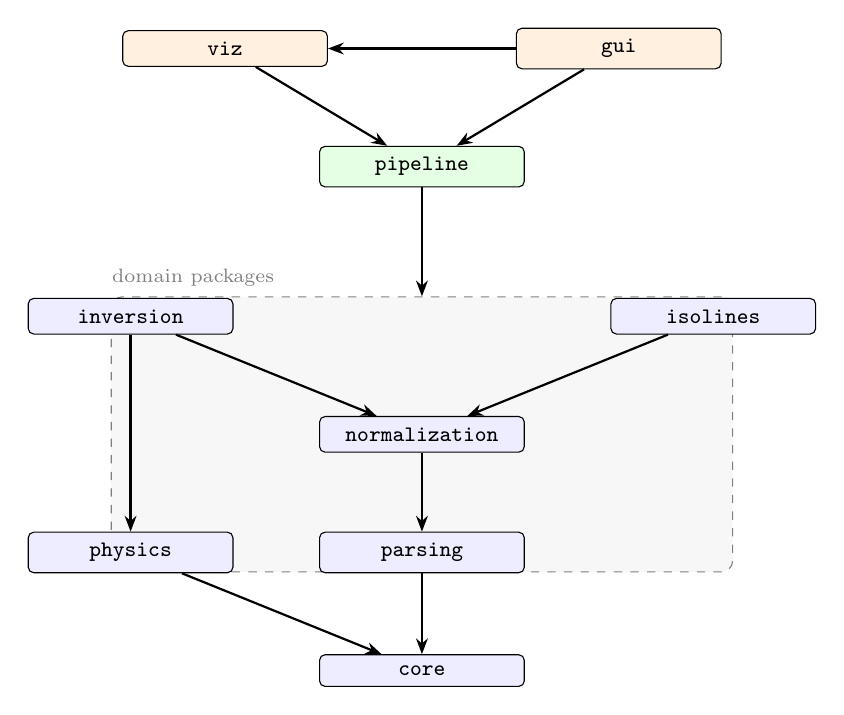
\begin{tikzpicture}[x=1cm, y=1cm]
\begin{scope}[on background layer]
  \node[draw=gray, dashed, rounded corners=4pt, fill=gray!6, inner sep=7pt,
        fit={(0.8,1.5) (8.2,4.5)}, label={[font=\scriptsize, gray]above
        left:domain packages}] (dom) {};
\end{scope}
\node[wbox, minimum width=2.6cm] (core) at (4.5,0) {\texttt{core}};
\node[wbox, minimum width=2.6cm] (parsing) at (4.5,1.5) {\texttt{parsing}};
\node[wbox, minimum width=2.6cm] (physics) at (0.8,1.5) {\texttt{physics}};
\node[wbox, minimum width=2.6cm] (norm) at (4.5,3.0) {\texttt{normalization}};
\node[wbox, minimum width=2.6cm] (iso) at (8.2,4.5) {\texttt{isolines}};
\node[wbox, minimum width=2.6cm] (inv) at (0.8,4.5) {\texttt{inversion}};
\node[wbox, minimum width=2.6cm, fill=green!10] (pipe) at (4.5,6.4)
  {\texttt{pipeline}};
\node[wbox, minimum width=2.6cm, fill=orange!12] (viz) at (2.0,7.9)
  {\texttt{viz}};
\node[wbox, minimum width=2.6cm, fill=orange!12] (gui) at (7.0,7.9)
  {\texttt{gui}};
\draw[arr] (parsing) -- (core);
\draw[arr] (physics) -- (core);
\draw[arr] (norm) -- (parsing);
\draw[arr] (iso) -- (norm);
\draw[arr] (inv) -- (norm);
\draw[arr] (inv) -- (physics);
\draw[arr] (pipe) -- (dom.north -| pipe);
\draw[arr] (viz) -- (pipe);
\draw[arr] (gui) -- (pipe);
\draw[arr] (gui) -- (viz);
\end{tikzpicture}
\caption{Allowed import directions (arrow = ``may import''). Isolines and
inversion consume the normalized sample; viz and gui only talk to the
pipeline.}
\label{fig:deps}
\end{figure}

\subsection{Data flow}
\label{sec:dataflow}

Figure~\ref{fig:flow} shows the complete flow from a CSV file to the plot.
Steps 2 to 5 are executed once for every parameter column.

\begin{figure}[htbp]
\centering
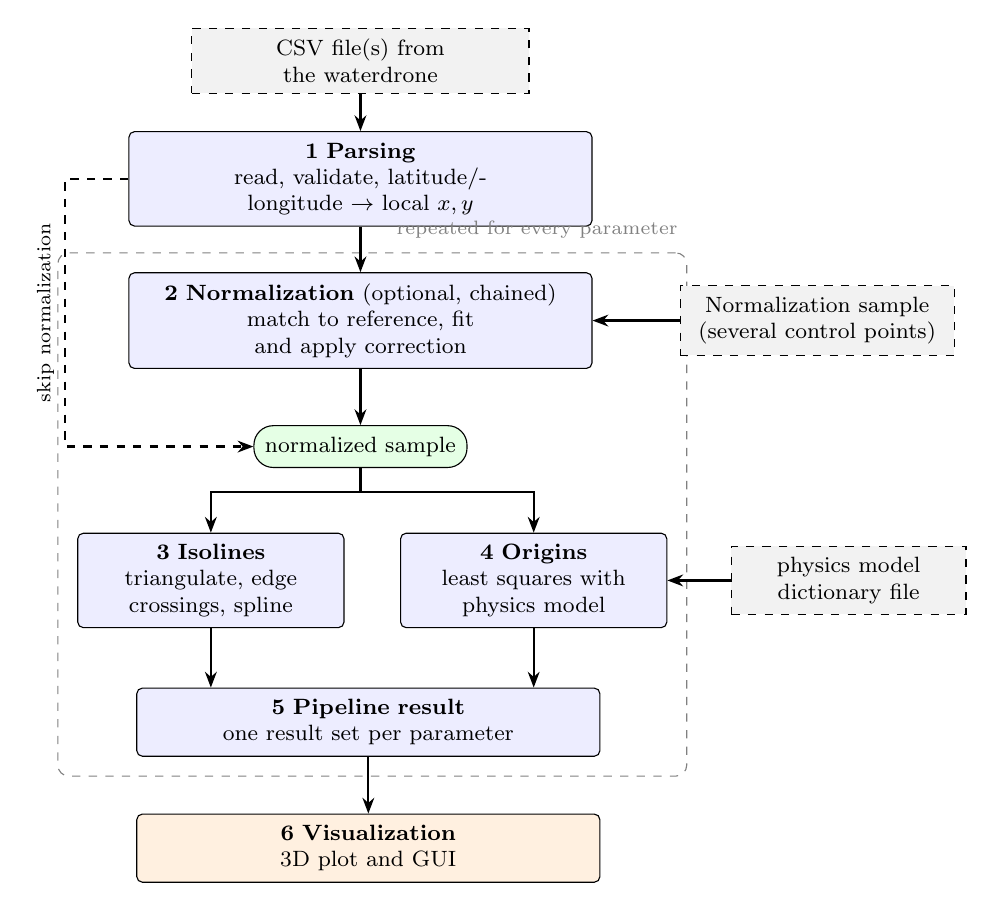
\begin{tikzpicture}[x=1cm, y=1cm]
\node[ext, text width=4cm] (csv) at (3.2,0) {CSV file(s) from the waterdrone};
\node[wbox, text width=5.6cm] (parse) at (3.2,-1.5)
  {\textbf{1~Parsing}\\ read, validate, latitude/longitude $\to$ local $x,y$};
\node[wbox, text width=5.6cm] (norm) at (3.2,-3.3)
  {\textbf{2~Normalization} (optional, chained)\\ match to reference, fit and
   apply correction};
\node[ext, text width=3.2cm] (ctrl) at (9.0,-3.3)
  {Normalization sample\\ (several control points)};
\node[dbox] (ns) at (3.2,-4.9) {normalized sample};
\node[wbox, text width=3.1cm] (iso) at (1.3,-6.6)
  {\textbf{3~Isolines}\\ triangulate, edge crossings, spline};
\node[wbox, text width=3.1cm] (inv) at (5.4,-6.6)
  {\textbf{4~Origins}\\ least squares with physics model};
\node[ext, text width=2.7cm] (phys) at (9.4,-6.6)
  {physics model dictionary file};
\node[wbox, text width=5.6cm] (pipe) at (3.3,-8.4)
  {\textbf{5~Pipeline result}\\ one result set per parameter};
\node[wbox, text width=5.6cm, fill=orange!12] (viz) at (3.3,-10.0)
  {\textbf{6~Visualization}\\ 3D plot and GUI};
\begin{scope}[on background layer]
  \node[draw=gray, dashed, rounded corners=4pt, inner sep=7pt,
        fit=(norm) (ns) (iso) (inv) (pipe)] (grp) {};
\end{scope}
\node[font=\scriptsize, gray, anchor=south east, yshift=1.5pt] at (grp.north east)
  {repeated for every parameter};
\draw[arr] (csv) -- (parse);
\draw[arr] (parse) -- (norm);
\draw[arr] (norm) -- (ns);
\draw[arr, dashed] (parse.west) -- ++(-0.8,0) |- (ns.west);
\node[font=\scriptsize, rotate=90] at (-0.8,-3.2) {skip normalization};
\draw[arr] (ctrl) -- (norm);
\draw[arr] (ns.south) -- ++(0,-0.3) -| (iso.north);
\draw[arr] (ns.south) -- ++(0,-0.3) -| (inv.north);
\draw[arr] (phys) -- (inv);
\draw[arr] (iso.south) -- (pipe.north -| iso.south);
\draw[arr] (inv.south) -- (pipe.north -| inv.south);
\draw[arr] (pipe) -- (viz);
\end{tikzpicture}
\caption{Data flow of the analysis app. Dashed grey boxes are inputs from
outside the pipeline; the dashed arrow shows that normalization may be
skipped.}
\label{fig:flow}
\end{figure}

\subsubsection*{Step 1 -- Parsing and coordinates}

\path{parsing/csv_parser.py} reads the file, finds the fixed columns and the
parameters, and rejects or flags invalid rows. \path{parsing/coordinates.py}
then converts latitude $\varphi$ and longitude $\lambda$ into local metres
around a shared reference point $(\varphi_0,\lambda_0)$. For a small area a
simple choice is
\begin{equation*}
  x = R\cos\varphi_0\,(\lambda-\lambda_0), \qquad y = R\,(\varphi-\varphi_0),
\end{equation*}
with angles in radians and $R$ the Earth radius. This formula is only an
illustration. The projection actually used, and the estimate of its error,
follow the team's lecture notes on coordinate systems, geographic coordinate
translation and error derivation (topic T3), which are kept outside the
repository. The reference origin is shared by all samples so that they
overlay correctly.

\subsubsection*{Step 2 -- Normalization (optional)}

A large survey takes a long time, so its readings mix spatial variation with
changes over time. A short survey of a few control points is nearly a
snapshot. Normalization uses such a snapshot as reference
(Figure~\ref{fig:chain}):

\begin{enumerate}
\item \path{matching.py} pairs points of the big sample with the reference by
      distance and by time and looks up reference values at arbitrary points
      through a spatial index.
\item \path{correction.py} fits a correction $g$ so that, on the matched
      pairs, the corrected reading $g(c_i,t_i;\boldsymbol\phi)$ agrees with
      the reference value $r_i$:
      \begin{equation*}
        \min_{\boldsymbol\phi}\sum_i\bigl(g(c_i,t_i;\boldsymbol\phi)-r_i\bigr)^2 ,
      \end{equation*}
      applies it to the whole sample and checks the residuals. The form of
      $g$ (offset, scale or time drift) is still an open decision
      (Section~\ref{sec:open}).
\item \path{chain.py} organises the samples as an ordered chain. A further,
      bigger sample is normalized against the \emph{previous normalized
      sample}, which then plays the role of the reference grid. The first
      step may be skipped when no control-point sample exists.
\end{enumerate}

Each parameter gets its own correction; they are never shared between
parameters.

\begin{figure}[htbp]
\centering
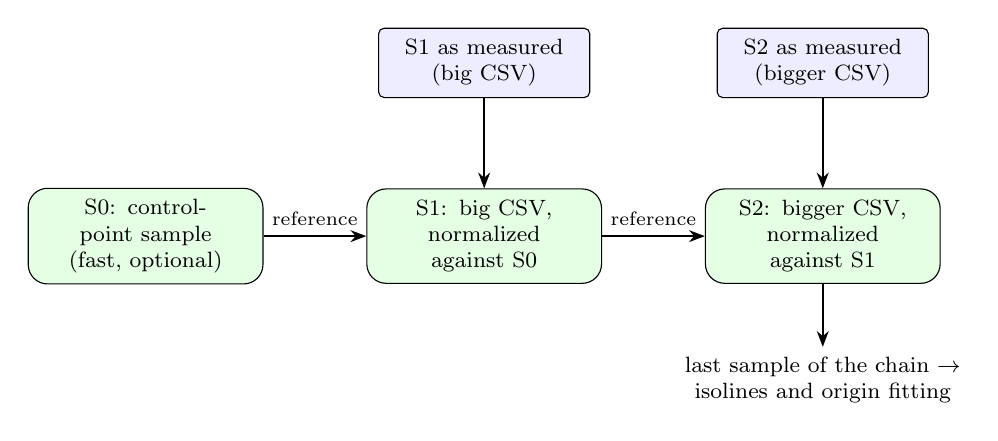
\begin{tikzpicture}[x=1cm, y=1cm]
\node[dbox, text width=2.7cm] (n0) at (1.5,0)
  {S0: control-point sample\\ (fast, optional)};
\node[dbox, text width=2.7cm] (n1) at (5.8,0)
  {S1: big CSV,\\ normalized\\ against S0};
\node[dbox, text width=2.7cm] (n2) at (10.1,0)
  {S2: bigger CSV,\\ normalized\\ against S1};
\node[wbox, text width=2.4cm] (r1) at (5.8,2.2) {S1 as measured\\ (big CSV)};
\node[wbox, text width=2.4cm] (r2) at (10.1,2.2)
  {S2 as measured\\ (bigger CSV)};
\draw[arr] (n0) -- node[above, font=\scriptsize] {reference} (n1);
\draw[arr] (n1) -- node[above, font=\scriptsize] {reference} (n2);
\draw[arr] (r1) -- (n1);
\draw[arr] (r2) -- (n2);
\draw[arr] (n2.south) -- ++(0,-0.8)
  node[below, font=\footnotesize, align=center]
  {last sample of the chain $\to$\\ isolines and origin fitting};
\end{tikzpicture}
\caption{A normalization chain with two links. Each normalized sample becomes
the reference grid of the next one; the chain can be longer.}
\label{fig:chain}
\end{figure}

\subsubsection*{Step 3 -- Triangulation and isolines}

\path{isolines/triangulation.py} triangulates the normalized sample and drops
triangles that bridge gaps in the track or span land. For each isoline level
$L$, \path{contours.py} inspects every triangle edge whose end values $v_1$
and $v_2$ lie on different sides of $L$. The crossing lies at
\begin{equation*}
  \mathbf{p} = \mathbf{p}_1 + t\,(\mathbf{p}_2-\mathbf{p}_1),\qquad
  t = \frac{L-v_1}{v_2-v_1}.
\end{equation*}
The crossings of one triangle are connected by a segment, the segments of
neighbouring triangles are linked into polylines, and a spline smooths each
polyline (Figure~\ref{fig:tri}). Levels and smoothing come from
\path{defaults.txt} unless the user changes them.

\begin{figure}[htbp]
\centering
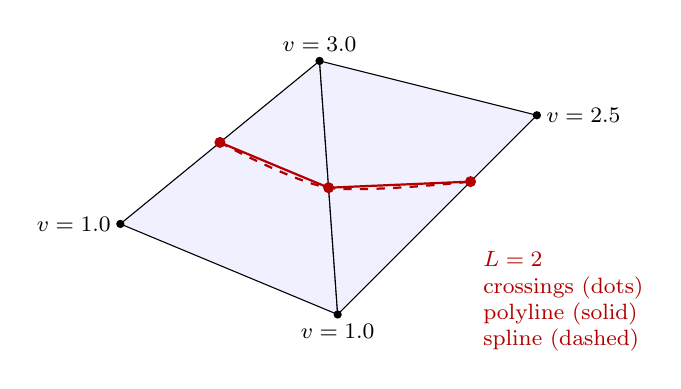
\begin{tikzpicture}[x=1.15cm, y=1.15cm, font=\footnotesize]
\coordinate (A) at (0,1.0);
\coordinate (B) at (2.2,2.8);
\coordinate (C) at (2.4,0);
\coordinate (D) at (4.6,2.2);
\draw[fill=blue!6] (A) -- (B) -- (C) -- cycle;
\draw[fill=blue!6] (B) -- (C) -- (D) -- cycle;
\coordinate (p1) at ($(A)!0.5!(B)$);
\coordinate (p2) at ($(B)!0.5!(C)$);
\coordinate (p3) at ($(C)!0.667!(D)$);
\draw[red!70!black, thick] (p1) -- (p2) -- (p3);
\draw[red!70!black, thick, dashed] plot[smooth] coordinates {(p1) (p2) (p3)};
\foreach \p in {p1,p2,p3} \fill[red!70!black] (\p) circle (2pt);
\foreach \p/\v/\pos in {A/1.0/left, B/3.0/above, C/1.0/below, D/2.5/right}
  \node[\pos] at (\p) {$v=\v$};
\foreach \p in {A,B,C,D} \fill (\p) circle (1.5pt);
\node[red!70!black, anchor=north west, align=left] at (3.9,0.8)
  {$L=2$\\ crossings (dots)\\ polyline (solid)\\ spline (dashed)};
\end{tikzpicture}
\caption{Two neighbouring triangles with vertex values. For the level
$L=2$ the isoline crosses three edges, at $t=0.5$ on the first two and
$t\approx0.67$ on the third; the crossings are linked and smoothed.}
\label{fig:tri}
\end{figure}

\subsubsection*{Step 4 -- Origin finding}

\path{physics/spec.py} reads the dictionary text file and tells the solver
which physics model belongs to which CSV parameter, with bounds.
\path{physics/models.py} implements the forward models. For a model $f$ and a
set of $K$ origins described by parameters $\boldsymbol\theta$, the solver in
\path{inversion/fit.py} minimizes the sum of squared residuals over the
normalized sample points $(x_i,y_i)$ with values $c_i$:
\begin{equation*}
  \min_{\boldsymbol\theta}\sum_i\bigl(c_i - f(x_i,y_i;\boldsymbol\theta)\bigr)^2
  \quad\text{subject to the bounds from the dictionary.}
\end{equation*}
\path{inversion/diagnostics.py} then reports the RMS error, a residual map
and a sanity check of the number of origins. For synthetic samples it also
compares the result with the known origins.

An illustrative (not final) dictionary file could look like this; the real
format is fixed when \path{physics/spec.py} is written.

\begin{lstlisting}
# PARAMETER   MODEL
PARAM_A       model_one
PARAM_B       model_two
\end{lstlisting}

\subsubsection*{Step 5 and 6 -- Pipeline and visualization}
\label{sec:viz}

\path{pipeline/stages.py} wraps steps 1--4 as stages, \path{run.py} runs them
for one or all parameters and caches the results, and \path{state.py} keeps
the immutable application state. \path{viz/plot3d.py} draws a matplotlib 3D
plot whose horizontal axes are the local coordinates $x,y$ in metres and
whose vertical axis is the \emph{parameter value}. (The CSV column \texttt{Z}
is measurement depth and is not used as the vertical axis.)
\path{viz/overlays.py} adds isolines and origins on request.

\subsection{How it will look on screen}
\label{sec:screens}

The GUI is a single window; the toolkit is likely Tkinter and is isolated in
\path{gui/} so it can be exchanged. Figure~\ref{fig:window} is a mock-up with
invented data and file names.

\begin{figure}[htbp]
\centering
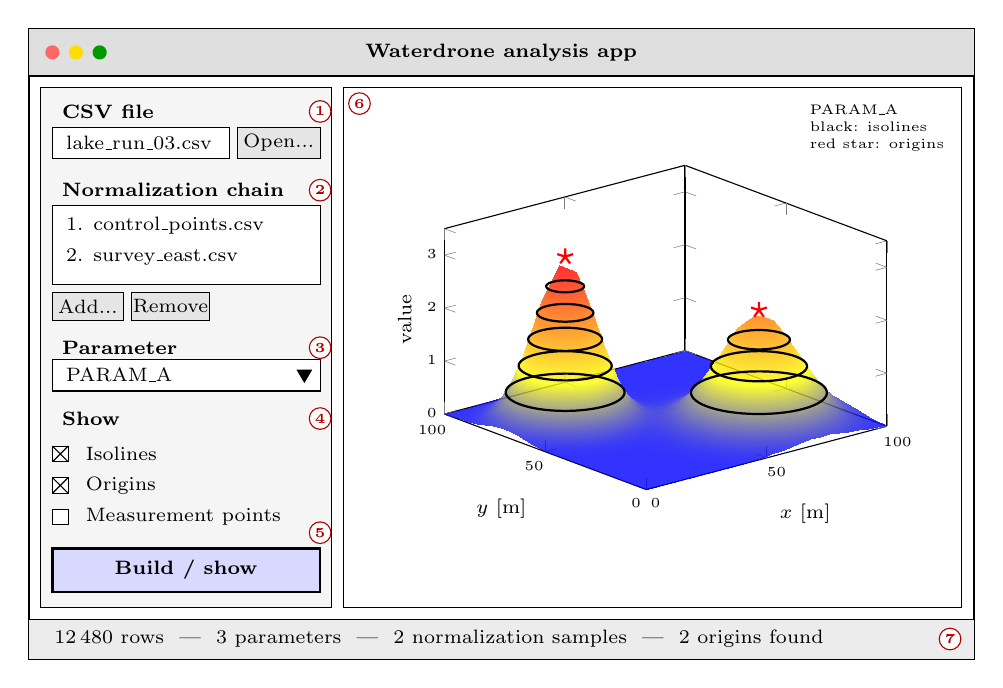
\begin{tikzpicture}[x=1cm, y=1cm, font=\scriptsize]
% window frame and title bar
\draw[thick, fill=white] (0,0) rectangle (12,8);
\fill[gray!25] (0,7.4) rectangle (12,8);
\draw (0,7.4) -- (12,7.4);
\node at (6,7.7) {\textbf{Waterdrone analysis app}};
\fill[red!60] (0.3,7.7) circle (0.09);
\fill[yellow!80!orange] (0.6,7.7) circle (0.09);
\fill[green!60!black] (0.9,7.7) circle (0.09);
% control panel
\draw[fill=gray!8] (0.15,0.65) rectangle (3.85,7.25);
\node[anchor=west] at (0.3,6.95) {\textbf{CSV file}};
\draw[fill=white] (0.3,6.35) rectangle (2.55,6.75);
\node[anchor=west] at (0.35,6.55) {lake\_run\_03.csv};
\draw[fill=gray!20] (2.65,6.35) rectangle (3.7,6.75);
\node at (3.175,6.55) {Open...};
\node[anchor=west] at (0.3,5.95) {\textbf{Normalization chain}};
\draw[fill=white] (0.3,4.75) rectangle (3.7,5.75);
\node[anchor=west] at (0.35,5.5) {1. control\_points.csv};
\node[anchor=west] at (0.35,5.1) {2. survey\_east.csv};
\draw[fill=gray!20] (0.3,4.3) rectangle (1.2,4.65);
\node at (0.75,4.475) {Add...};
\draw[fill=gray!20] (1.3,4.3) rectangle (2.3,4.65);
\node at (1.8,4.475) {Remove};
\node[anchor=west] at (0.3,3.95) {\textbf{Parameter}};
\draw[fill=white] (0.3,3.4) rectangle (3.7,3.8);
\node[anchor=west] at (0.35,3.6) {PARAM\_A};
\fill (3.4,3.67) -- (3.6,3.67) -- (3.5,3.5) -- cycle;
\node[anchor=west] at (0.3,3.05) {\textbf{Show}};
\draw[fill=white] (0.3,2.5) rectangle (0.5,2.7);
\draw (0.3,2.5) -- (0.5,2.7) (0.3,2.7) -- (0.5,2.5);
\node[anchor=west] at (0.6,2.6) {Isolines};
\draw[fill=white] (0.3,2.1) rectangle (0.5,2.3);
\draw (0.3,2.1) -- (0.5,2.3) (0.3,2.3) -- (0.5,2.1);
\node[anchor=west] at (0.6,2.2) {Origins};
\draw[fill=white] (0.3,1.7) rectangle (0.5,1.9);
\node[anchor=west] at (0.6,1.8) {Measurement points};
\draw[fill=blue!15, thick] (0.3,0.85) rectangle (3.7,1.4);
\node at (2.0,1.125) {\textbf{Build / show}};
% plot area
\draw (4.0,0.65) rectangle (11.85,7.25);
\node at (7.95,3.95) {\hillThreeD{7.2cm}{5.7cm}};
\node[anchor=north east, align=left, font=\tiny] at (11.75,7.15)
  {PARAM\_A\\ black: isolines\\ red star: origins};
% status bar
\fill[gray!15] (0,0) rectangle (12,0.5);
\draw (0,0.5) -- (12,0.5);
\node[anchor=west] at (0.2,0.25)
  {12\,480 rows \ | \ 3 parameters \ | \ 2 normalization samples \ | \ 2 origins found};
% call-outs
\node[call] at (3.7,6.95) {1};
\node[call] at (3.7,5.95) {2};
\node[call] at (3.7,3.95) {3};
\node[call] at (3.7,3.05) {4};
\node[call] at (3.7,1.6) {5};
\node[call] at (4.2,7.05) {6};
\node[call] at (11.7,0.25) {7};
\end{tikzpicture}
\caption{Mock-up of the main window with invented data: (1)~CSV picker,
(2)~normalization chain, (3)~parameter dropdown, (4)~display toggles,
(5)~build button, (6)~3D plot, (7)~status bar.}
\label{fig:window}
\end{figure}

A typical session is expected to run as follows.

\begin{enumerate}
\item The user picks a CSV file with the CSV picker (1). It is parsed and
      converted to local coordinates immediately.
\item Optionally, the user adds a control-point sample and further samples
      to the normalization list (2). The order in the list is the order of
      the chain.
\item The user selects a parameter in the dropdown (3) and presses
      \emph{Build / show} (5). The pipeline computes all parameters; the
      selected one is drawn.
\item Isolines and origins can be toggled (4). Switching the dropdown shows
      another parameter without recomputation, because all parameters were
      already computed (or are cached).
\item The 3D plot (6) can be rotated and zoomed with the usual matplotlib
      tools; the status bar (7) reports row counts and what was found.
\end{enumerate}

Figure~\ref{fig:render} shows what the plot is meant to convey: the field as
a surface over the local $x,y$ plane, isolines at fixed levels, the origins
the least-squares fit found, and, in the top view, the drone track that
produced the data. The field in this picture is two invented smooth hills,
not a measurement.

\begin{figure}[htbp]
\centering
\begin{minipage}{0.55\textwidth}
\centering
\hillThreeD{6.6cm}{5.6cm}\\[1mm]
\footnotesize (a) 3D view
\end{minipage}\hfill
\begin{minipage}{0.43\textwidth}
\centering
\hillTwoD{4.9cm}\\[1mm]
\footnotesize (b) top view with drone track (grey)
\end{minipage}
\caption{Possible render of one parameter (synthetic field): isolines in black,
fitted origins as red stars.}
\label{fig:render}
\end{figure}

\subsection{Adding a physics model}

Because the solver reads the model from the dictionary, a new model needs only
two edits:

\begin{enumerate}
\item add a forward-model function to \path{physics/models.py};
\item add a dictionary entry that maps a parameter to the new model name (and
      its bounds).
\end{enumerate}

The synthetic-sample scripts of phase~1 use the same function, so a new model
can be checked on generated data straight away.

% =====================================================================
\section{Test flow}
\label{sec:tests}

The analysis app has no \path{tests/} folder. All testing is done with the
repository-level \path{samples/} folder, in three phases that grow in
difficulty (Figure~\ref{fig:tests}). Because \path{pipeline/} contains no GUI
code, a script in \path{samples/} can run a sample through the same stages
the GUI uses.

\begin{figure}[htbp]
\centering
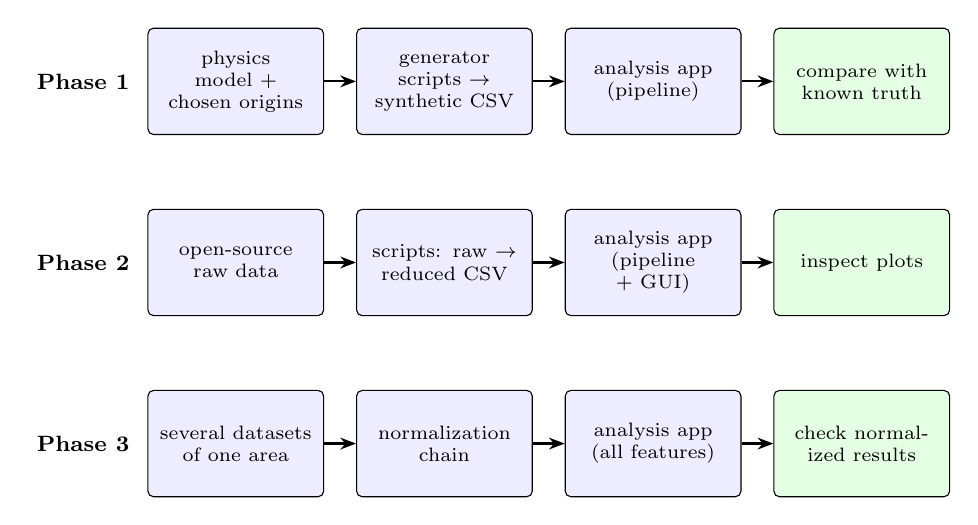
\begin{tikzpicture}[x=1cm, y=1cm]
\tikzset{tb/.style={wbox, text width=1.95cm, minimum height=1.35cm,
                    font=\scriptsize}}
\foreach \y/\lab in {0/Phase 1, -2.3/Phase 2, -4.6/Phase 3}
  \node[font=\footnotesize\bfseries, anchor=west] at (0,\y) {\lab};
% phase 1
\node[tb] (a1) at (2.65,0) {physics model + chosen origins};
\node[tb] (a2) at (5.3,0) {generator scripts $\to$ synthetic CSV};
\node[tb] (a3) at (7.95,0) {analysis app (pipeline)};
\node[tb, fill=green!10] (a4) at (10.6,0) {compare with known truth};
% phase 2
\node[tb] (b1) at (2.65,-2.3) {open-source raw data};
\node[tb] (b2) at (5.3,-2.3) {scripts: raw $\to$ reduced CSV};
\node[tb] (b3) at (7.95,-2.3) {analysis app (pipeline + GUI)};
\node[tb, fill=green!10] (b4) at (10.6,-2.3) {inspect plots};
% phase 3
\node[tb] (c1) at (2.65,-4.6) {several datasets of one area};
\node[tb] (c2) at (5.3,-4.6) {normalization chain};
\node[tb] (c3) at (7.95,-4.6) {analysis app (all features)};
\node[tb, fill=green!10] (c4) at (10.6,-4.6) {check normalized results};
\foreach \a/\b in {a1/a2,a2/a3,a3/a4,b1/b2,b2/b3,b3/b4,c1/c2,c2/c3,c3/c4}
  \draw[arr] (\a) -- (\b);
\end{tikzpicture}
\caption{The three test phases. Each lane shows where the data comes from and
what is checked at the end.}
\label{fig:tests}
\end{figure}

\subsection{Phase 1 -- synthetic samples}

\textbf{Folder:} \path{samples/phase1_synthetic/} (generator scripts in
\path{scripts/}).

\textbf{Idea.} The samples are \emph{abstract}: they are generated with the
same physics model that is pre-configured in the app. A script chooses origins
with known positions, evaluates the forward model from
\path{analysis_app.physics} along a track, and writes a CSV file in the
waterdrone format. The truth is therefore known exactly.

\textbf{What it checks.} The \emph{correctness} of the app. For example:
parsing and coordinate conversion, whether the isolines lie where the model
says they should, and above all whether the least-squares fit recovers the
known origins (\path{inversion/diagnostics.py} compares the result with them).
Variants such as gaps in the track can be generated to exercise the handling
of triangles that bridge gaps. Acceptance thresholds are still to be agreed.

\subsection{Phase 2 -- real-world data}

\textbf{Folder:} \path{samples/phase2_real/} with three subfolders:

\begin{itemize}
\item \path{raw/} -- open-source data as downloaded (the Utah Lake data is the
      first data set);
\item \path{reduced/} -- the same data converted to the waterdrone CSV format,
      keeping only concentration-related parameters;
\item \path{scripts/} -- the conversion scripts from \path{raw/} to
      \path{reduced/}.
\end{itemize}

\textbf{What it checks.} The \emph{visualization} on real data: how the 3D plot,
isolines and overlays behave with real tracks, noise and irregular coverage.
There are no known origins here, so quality is judged by inspecting the plots.

\subsection{Phase 3 -- normalization and extra features}

\textbf{Folder:} \path{samples/phase3_normalization/} -- not created yet.

\textbf{Idea.} The ultimate test. It uses the extra features, above all the
normalization of data with the help of several different data sets, so the
whole normalization chain (Figure~\ref{fig:chain}) is exercised end to end,
and the normalized result then feeds isolines and origin fitting.

\textbf{What it checks.} That the app works with several data sets of one
area at once. The data sets and acceptance criteria are still to be chosen.

\subsection{Summary}

\begin{center}
\begin{tabular}{@{}>{\raggedright\arraybackslash}p{0.09\textwidth}>{\raggedright\arraybackslash}p{0.28\textwidth}>{\raggedright\arraybackslash}p{0.26\textwidth}>{\raggedright\arraybackslash}p{0.26\textwidth}@{}}
\toprule
\textbf{Phase} & \textbf{Folder} & \textbf{Data} & \textbf{Main question}\\
\midrule
1 & \path{samples/phase1_synthetic/} & generated from the app's physics
  model & Is the app correct?\\
2 & \path{samples/phase2_real/} & open-source real data, reduced to the
  waterdrone format & Does the visualization work on real data?\\
3 & \path{samples/phase3_normalization/} (to be created) & several data
  sets of one area & Does normalization across data sets work?\\
\bottomrule
\end{tabular}
\end{center}

% =====================================================================
\section{Open decisions and where to start}
\label{sec:status}

\subsection{Open decisions}
\label{sec:open}

\begin{itemize}
\item \textbf{Normalization correction model.} Offset, scale or time drift?
      This must be decided before \path{normalization/correction.py} is
      written.
\item \textbf{Which sample feeds isolines and origin fitting.} The assumption
      is the last sample of the chain; the alternative is all samples merged.
\item \textbf{GUI toolkit.} Tkinter is the likely default; the choice is
      isolated in \path{gui/}.
\item \textbf{Physics model format and the first models.} The dictionary file
      format and the concrete models are not fixed yet.
\item \textbf{Phase 3 data sets and acceptance criteria}, as well as the
      thresholds for phases 1 and 2.
\end{itemize}

\subsection{Suggested starting point}

Following the dependency direction of Figure~\ref{fig:deps}, a natural order
for the first implementation is: \path{core}, then \path{parsing} and
\path{physics} (so that phase-1 samples can be generated early), then
\path{isolines}, \path{inversion} and \path{normalization}, then
\path{pipeline}, and finally \path{viz} and \path{gui}. Whatever you pick up,
keep to the rules of Section~\ref{sec:principles}: functions instead of
classes, one file per group of related functions, imports only through
package interfaces.

The second app, which configures the waterdrone, is planned for later and has
no structure yet.

\end{document}
